% Survey - lista preliminar da literatura -> validação com usuários reais, agregando novos requisitos
% protocolo, questionário, requisitos propostos, resultados, análise

%=============================
\chapter{Survey}\label{survey}
%=============================

In this chapter, more detailed information is presented about the survey that was conducted. Similar to the previous chapter, which talks about the grey literature systematic review, the survey was also a joined effort work between two authors. The tasks on which each was responsible will be described later. The \Cref{sec:survey-protocol}, presents details about the protocol created, author of reference and division of tasks among the researchers. Afterwards, in \Cref{sec:survey-validity}, threats to the validity of the study are reported. Finally, \Cref{sec:survey-results}, presents all results achieved during execution.

\section{Survey Protocol}\label{sec:survey-protocol}

A survey is an approach to data collection and analysis in which respondents answer questions or statements that were developed in advance. The protocol chosen for the elaboration of this study was inspired by the guidelines proposed by \citeonline{kasunic2005designing}, in \textit{Designing an effective survey} and is illustrated in \Cref{fig:setepassos}.

\begin{figure}[!htb]
  \caption{Seven Steps of the Research Process}\label{fig:setepassos}
  \begin{center}
    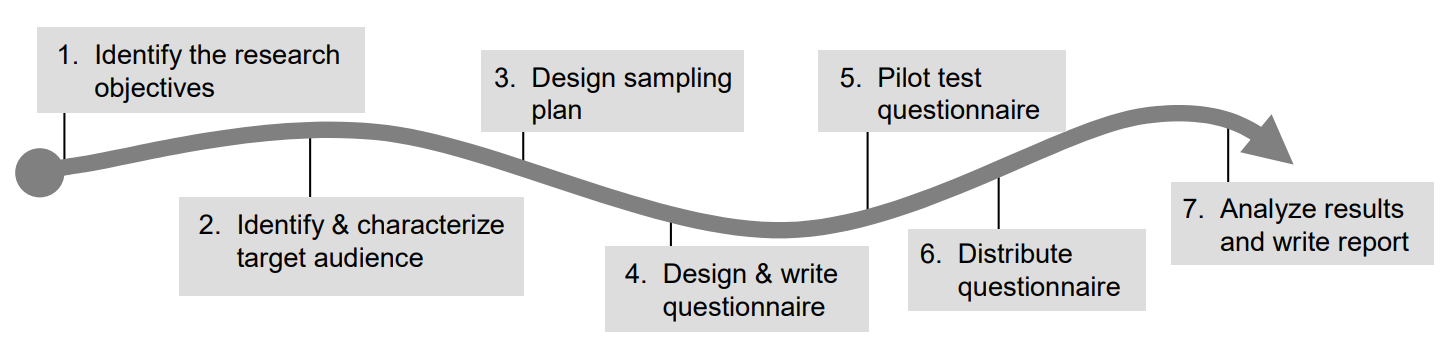
\includegraphics[width=16cm]{img/kasunic_process.png}
  \end{center}
  \fonte{\cite{kasunic2005designing}.}
\end{figure}

As will be described in more detail later, the objective is to understand the needs of students and teachers in relation to projects and outreach activities. The choice of a survey as a data collection approach is due to the fact that according to \citeonline{kasunic2005designing}, the characteristics of such a research allows us to generalize about the beliefs and opinions of many people studying only a subset of them. Which is the perfect fit for this study.

Given that this research was performed by two students, the effort was divided equally, so that quality and performance were improved. \Cref{tbl:survey-tasks} describes the division of activities created by the authors and also already includes those defined by \citeonline{kasunic2005designing}.

\begin{table}
  \centering
  \caption{Tasks Separation}
  \label{tbl:survey-tasks}
  \footnotesize
  \begin{tabular}{l|l}
    \bottomrule
    \rowcolor[rgb]{0.753,0.753,0.753} \multicolumn{1}{c|}{\textbf{Activity}}                             & \multicolumn{1}{c}{\textbf{Responsibility}} \\
    \hline
    \rowcolor[rgb]{0.898,0.898,0.898} Define and document research objectives                            & Lucas F.                                    \\
    Define and document research questions                                                               & Lucas F.                                    \\
    \rowcolor[rgb]{0.898,0.898,0.898} Define and document how research results will be used              & Lucas F.                                    \\
    Define the appropriate target audience for the research                                              & Igor C.                                     \\
    \rowcolor[rgb]{0.898,0.898,0.898} Determine the appropriate media to apply the research in           & Igor C.                                     \\
    Recruit members of the target audience to participate in pilot test                                  & Igor C.                                     \\
    \rowcolor[rgb]{0.898,0.898,0.898} Breakdown research questions into questionnaire topics             & Lucas F.                                    \\
    Organize and sequence questions                                                                      & Lucas F.                                    \\
    \rowcolor[rgb]{0.898,0.898,0.898} Review the questionnaire based on the pilot test                   & Igor C. and Lucas F.                        \\
    Perform the pilot test                                                                               & Igor C. and Lucas F.                        \\
    \rowcolor[rgb]{0.898,0.898,0.898} Evaluate comments                                                  & Igor C. and Lucas F.                        \\
    Perform final corrections before the distribution of the questionnaire                               & Lucas F.                                    \\
    \rowcolor[rgb]{0.753,0.753,0.753} \multicolumn{1}{c|}{\textbf{Questionnaire ready for distribution}} &                                             \\
    Distribute questionnaires                                                                            & Lucas F.                                    \\
    \rowcolor[rgb]{0.898,0.898,0.898} Monitor answers                                                    & Igor C. and Lucas F.                        \\
    Send reminders                                                                                       & Igor C.                                     \\
    \rowcolor[rgb]{0.753,0.753,0.753} \multicolumn{1}{c|}{\textbf{Questionnaire response deadline}}      &                                             \\
    Perform analysis                                                                                     & Igor C. and Lucas F.                        \\
    \rowcolor[rgb]{0.898,0.898,0.898} Write draft report                                                 & Igor C.                                     \\
    Revise draft                                                                                         & Igor C. and Lucas F.                        \\
    \rowcolor[rgb]{0.898,0.898,0.898} Perform the final corrections                                      & Igor C. and Lucas F.                        \\
    \toprule
  \end{tabular}
\end{table}

\subsection{Identify the Research Objectives}\label{sec:survey-objectives}

The point of having well defined research objectives, as \citeonline[p. 13]{kasunic2005designing} presents, is to increase the odds of executing a successful questionnaire. Through the results generated by the grey literature systematic review, mentioned earlier in \Cref{greyliterature}, it was possible to elaborate questions so that the participant informs, in his view, the importance of a certain requirement. This survey aims to order by priority and refine the elicited requirements, using the individual opinion the target audience.

In addition to being asked the participants' opinion, they were also allowed to provide long written feedbacks and suggestions or improvements to each of the presented requirements. Since one of the objectives of the survey was to refine existing requirements, enabling the users to describe their thoughts in more detail allowed the authors to identify underlying issues that would otherwise go unnoticed.

\subsection{Identify and Characterize the Target Audience}\label{sec:survey-targets}

\subsection{Design the Sampling Plan}\label{sec:survey-sampling}

\subsection{Design and Write the Questionnaire}\label{sec:survey-questionnaire}

\subsubsection{The Welcome Screen}

\subsubsection{Profile Questions}\label{survey:profile-questions}

\subsubsection{Requirements Priorization Questions}

\subsubsection{Feature suggestions}

\subsection{Pilot Questionnaire}\label{sec:survey-pilot}

As \citeonline[p. 75]{kasunic2005designing} describes, a pilot test is a simulation of the real questionnaire carried out with a small number of members from the target audience. For this, the authors hand picked 7 (seven) people, out of which 4 (four) were students, 2 (two) were professors and 1 (one) was an \acl{TAE} (\ac{TAE}). The reason behind choosing this specific number of respondents is due to the following:
\begin{inparaenum}[(i)]
  \item All defined profiles for the respondents were chosen and
  \item the ratio of 4/2/1 is aligned with the expected numbers of submitted questionnaires per profile.
\end{inparaenum}

Unfortunately, the person chosen for the third profile, \ac{TAE}, wasn't able to answer. However, even though there are 3 (three) profiles, the questionnaire itself only has 2 (two) tracks of questions, one for students and the other for professors/\acp{TAE}. Because of that, the consequences of this happening weren't too impactful.

As for the pilot results, a lot of great feedback was received, along with some compliments on the organization of the questionnaire. There were issues with the person identification section, where the age was changed from a number to a range of numbers, such as between 21-29 years old.

\subsection{Distribute the Questionnaire}\label{sec:survey-distribute}

\subsection{Analyze the Results and Write a Report}\label{sec:survey-analyse}

\section{Threats to validity}\label{sec:survey-validity}

% TAE didn't answer pilot test

\section{Results}\label{sec:survey-results}